%% Autor: Björn Ritterbecks 
%% Letzte Aenderung: 15.06.2016 
\thisfloatsetup{%
  capbesidewidth=\marginparwidth}
\begin{figure}[htbp]
\centering
%\sansmath
 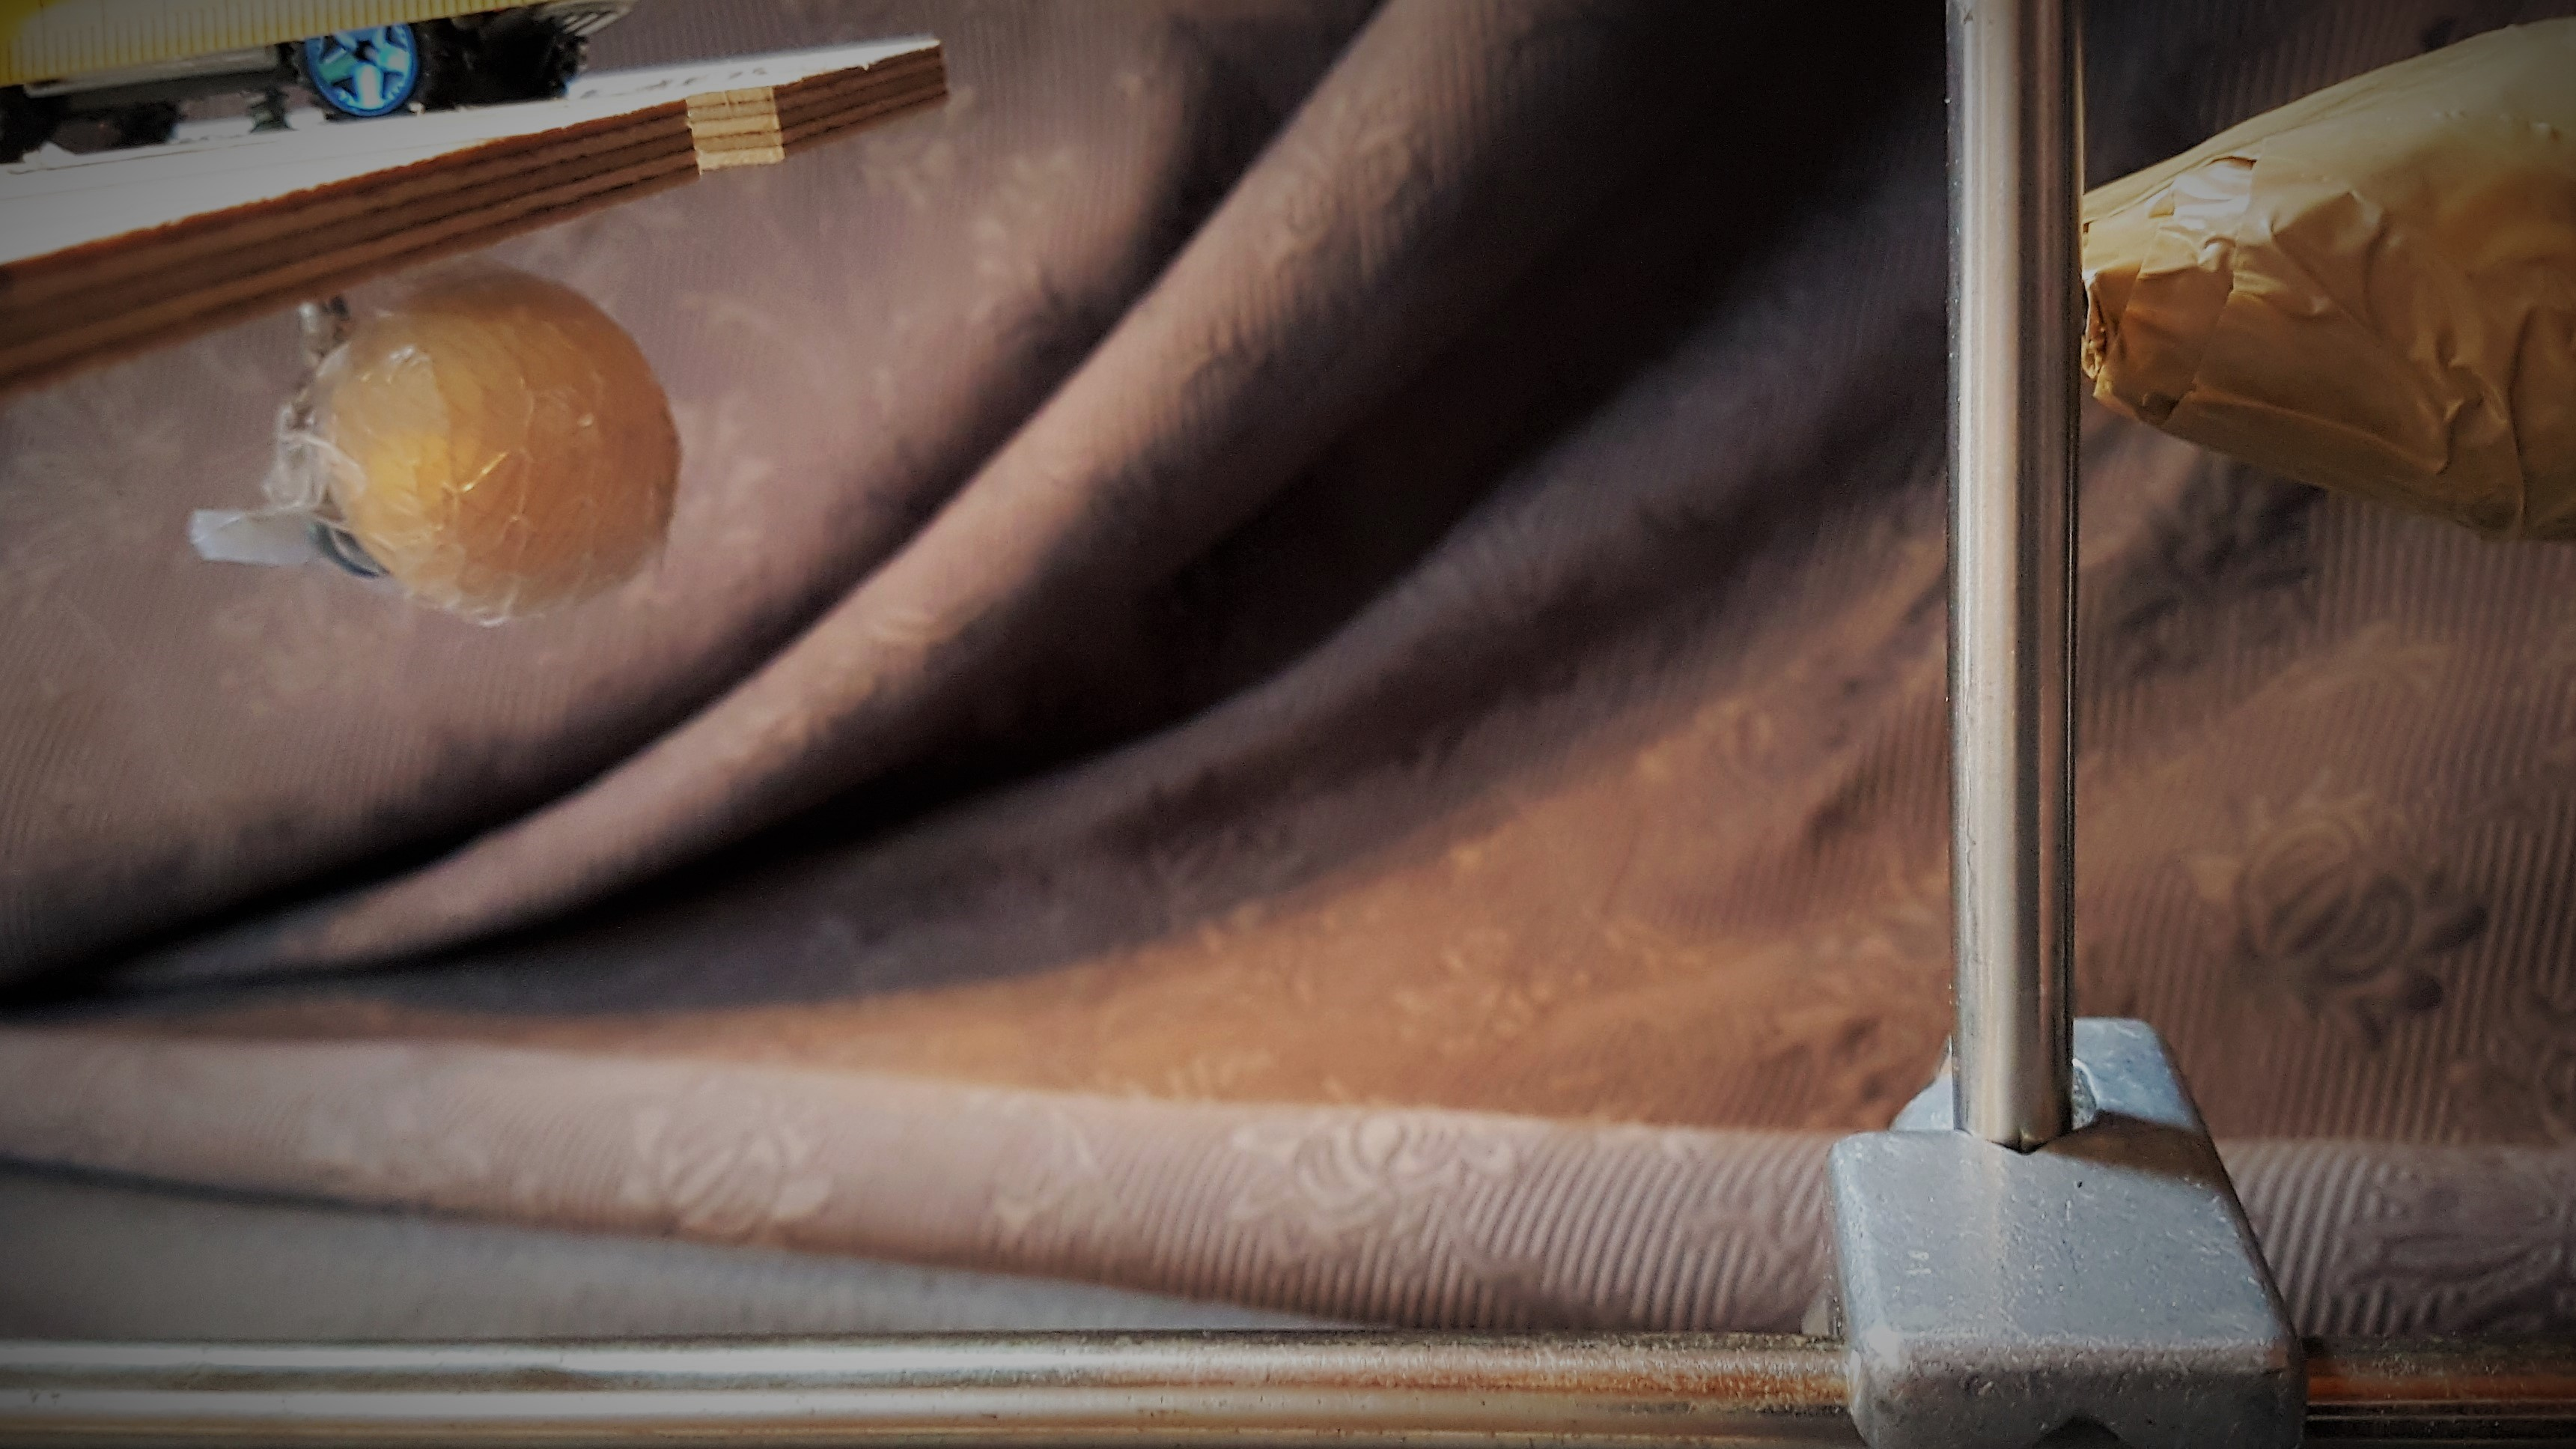
\includegraphics[width=0.99\textwidth]{images/stroemungskraftmessung2.jpg}
  \caption[Analogieversuch zu Massenspektrometrie nach \textsc{Luchner}, \textsc{Degner} und \textsc{Schilling} ]{Funktionsmodell eines Massenspektrometers der Nuffield Foundation. Kugellager-Kugeln rollen durch ein Glasrohr nach unten auf die Platte, wo sie von einem Magneten gestreut werden. Die leichtesten Kugeln werden am Weitesten abgelenkt (entnommen aus \cite[S\,262]{Nuffield1970}).}
  \label{fig:stroemungskraftmessung2}
  \vspace{-0pt}
\end{figure}